\documentclass[12pt, openany]{report}
\usepackage[utf8]{inputenc}
\usepackage[T1]{fontenc}
\usepackage{amsmath,amsfonts,amssymb}
\usepackage{amssymb}
\usepackage{multicol}
\usepackage[a4paper,left=2.5cm,right=2.5cm,top=2.5cm,bottom=2.5cm]{geometry}
\usepackage[english]{babel}
\usepackage{libertine}
\usepackage{graphicx}
\usepackage{wrapfig}
\usepackage{algorithm}
\usepackage{algpseudocode}
\usepackage{float}
\usepackage{enumitem}
\usepackage{pythonhighlight}
\usepackage[]{titletoc}
\usepackage{empheq}
\usepackage{titlesec}
\usepackage{mathpazo}
\usepackage{xfrac}
\usepackage{textcomp}
\usepackage{mathtools}
\usepackage{caption}
\usepackage{tabularray}
\usepackage{subcaption}
\usepackage[bottom]{footmisc}
\usepackage{pdfpages}
\usepackage{tabularx}
\usepackage{amsthm}
\usepackage[skins]{tcolorbox}
\titleformat{\chapter}[display]
  {\normalfont\bfseries}{}{0pt}{\Huge}
\usepackage{hyperref}
\newcommand{\hsp}{\hspace{20pt}}
\newcommand{\HRule}{\rule{\linewidth}{0.5mm}}
\newcommand{\R}{\mathbb{R}}
\newcommand{\C}{\mathbb{C}}
\renewcommand{\P}{\mathbb{P}}
\newcommand{\A}{\mathcal{A}}
\newcommand{\Z}{\mathbb{Z}}
\newcommand{\E}{\mathbb{E}}
\theoremstyle{definition}
\newtheorem{thm}{Theorem}[chapter]
\newtheorem{definition}[thm]{Definition}
\newtheorem{lem}[thm]{Lemma}

\hbadness=100000
\begin{document}
\begin{titlepage}
    \begin{sffamily}
    \begin{center}
        
\includegraphics[scale=0.25]{img/page_de_garde.png} \\[1cm]
        \HRule \\[0.4cm]
        { \huge \bfseries LINMA2491 Operational Research \\[0.4cm] }
    
        \HRule \\[1.5cm]
        \textsc{\LARGE Simon Desmidt\\ Issambre L'Hermite Dumont}\\[1cm]
        \vfill
        \vspace{2cm}
        {\large Academic year 2024-2025 - Q2}
        \vspace{0.4cm}
         
        
\includegraphics[width=0.15\textwidth]{img/epl.png}
        
        UCLouvain\\
    
    \end{center}
    \end{sffamily}
\end{titlepage}

\setcounter{tocdepth}{1}
\tableofcontents
\chapter{Definition and notation}
\begin{itemize}
	\item Given $\Omega$, a sigma-algebra $\A$ is a set of subsets of $\Omega$, with the elements called events, such that:
	\begin{itemize}
		\item $\Omega \in \A$
		\item if $A \in \A$ then also $\Omega - A \in \A$
		\item if $A_i \in \A$ for $i = 1,2, \dots$ then also $\cup_{i=1}^\infty A_i \in \A$
		\item if $A_i \in \A$ for $i = 1,2, \dots$ then also $\cap_{i=1}^\infty A_i \in \A$
	\end{itemize}
	\item Consider: 
	\begin{figure}[H]
		\centering
		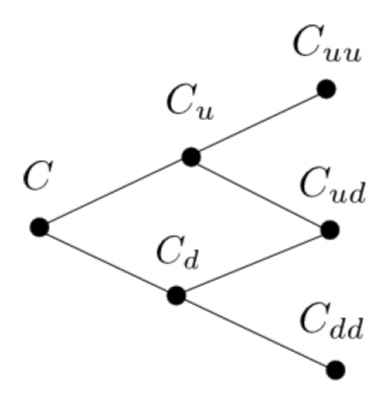
\includegraphics[scale=0.25]{img/space.jpg} 
	\end{figure}
	\begin{itemize}
		\item The state space is the set of all values of the system at each stage. 
		\begin{equation}
			S_0 = \{C\},\qquad S_1 = \{C_u, C_d\},\qquad S_2 = \{C_{uu}, C_{ud}, C_{dd}\}
		\end{equation}
		\item  The sample space is the set of all possible combination of the system.
		\begin{equation}
			\Omega = S_0 \times S_1 \times S_2 = \{(C, C_u, C_{uu}), (C, C_u, C_{ud}), (C, C_u, C_{dd}), \dots\}
		\end{equation}
	\end{itemize}
	\item The power set of $\Omega$ is the set of all of the subsets, denoted $\mathcal{B}(\Omega)$.
	\item The probability space is the triplet $(\Omega, \A, P)$ where $P$ is a probability measure.
	\begin{itemize}
		\item $P(\emptyset) = 0$
		\item $P(\Omega) = 1$
		\item $P(\cup_{i=1}^\infty A_i) = \sum_i P(A_i)$ if $A_i$ are disjoint
	\end{itemize} 
	\item $\forall t, A_t$ is the set of events on which we have information at stage $t$. For example, $A_0 = \{C\}$, $A_1 = \{C, C_u, C_d\}$. Thus is it evident that $ t_1 \leq t_2 \Rightarrow \A_{t_1} \subseteq \A_{t_2}$
	\item Consider the following problem with $x \in \R^n$ and domain $\mathcal{D}$:
	\begin{equation}
		\begin{aligned}
			&\min f_0(x), \qquad s.t.\\
			&f_i(x) \leq 0, i = 1, \dots, m\\
			&h_j(x) = 0, j = 1, \dots, p
		\end{aligned}
	\end{equation}
	Then the Lagrangian function is defined as $L: \R^n \times \R^m \times \R^p \to \R$:
	\begin{equation}
		L(x, \lambda, \nu) = f_0(x) + \sum_{i=1}^m \lambda_i f_i(x) + \sum_{j=1}^p \nu_j h_j(x)
	\end{equation}
	\item  The Lagrange dual function is defined as $g: \R^m \times \R^p \to \R$:
	\begin{equation}
		g(\lambda, \nu) = \inf_{x \in \mathcal{D}} L(x, \lambda, \nu)
	\end{equation}
	\item The Lagrange dual problem is a lower bound on the optimal value of the primal problem
	\item Lagrange relaxation of Stochastic Programs, consider the two problems:
	\begin{equation}
		\begin{aligned}
			\min f_1(x) + \E_\omega[f_2(y(\omega), \omega)] \qquad & \qquad \min f_1(x) + \E_\omega[f_2(y(\omega), \omega)]\\
			s.t \qquad h_{1i}(x) \leq 0, i = 1, \dots, m_1 \qquad & \qquad s.t. \qquad h_{1i}(x) \leq 0, i = 1, \dots, m_1\\
			h_{2i}(x,y(\omega),\omega) \leq 0, i = 1, \dots, m_2 \qquad & \qquad h_{2i}(x(\omega),y(\omega),\omega) \leq 0, i = 1, \dots, m_2\\
			& \textcolor{red}{\qquad x(\omega) = x} 
		\end{aligned}
	\end{equation}
	The red constraint is the non-anticipativity constraint, it transforms the deterministic variable into a stochastic variable. \textcolor{red}{A VERIFIER}
	\item The dual of a stochastic program is:
	\begin{equation}
		\begin{aligned}
			& g(\nu) = g1(\nu) + \E_\omega(g2(\nu, \omega))\\
			where \qquad &  \\
			& g_1(\nu) = \inf f_1(x) + \left( \displaystyle \sum_{\omega \in \Omega} \nu(\omega) \right)^T x\\
			& s.t. \quad h_{1i} (x) \leq 0, i = 1, \dots, m_1\\
			and \qquad &  \\
			& g_2(\nu, \omega) = \inf f_2(y(\omega) \omega) - \nu x(\omega)\\
			& s.t. \quad h_{2i}(x(\omega), y(\omega), \omega) \leq 0, i = 1, \dots, m_2
		\end{aligned}
	\end{equation}
	\item  With $p^*$ the solution of the primal problem and $d^*$ the solution of the dual problem, we have:
	\begin{itemize}
		\item Weak duality: $d^* \leq p^*$
		\item Strong duality: $d^* = p^*$
	\end{itemize}
	\item The KKT conditions are necessary and sufficient for optimality in convex optimization, there aren't unique. They are:
	\begin{itemize}
		\item Primal constraint: $f_i(x) \leq 0, i = 1, \dots, m$, $h_j(x) = 0, j = 1, \dots, p$
		\item Dual constraint: $\lambda \geq 0$
		\item Complemetarity slackness: $\lambda_i f_i(x) = 0, i = 1, \dots, m$
		\item Gradient of the Lagrangian: $\nabla_x L(x, \lambda, \nu) = 0$
	\end{itemize}
\end{itemize}
\chapter{Modelling}
\section{Introduction}
\begin{itemize}
	\item  For a certain sequence of events $x \to \omega \to y(\omega)$, where $\omega$ is the uncertainty,
	\begin{itemize}
		\item A first-stage decision is a decision that is made before the uncertainty is revealed (i.e. in $x$);
		\item A second-stage decision is a decision that is made after the uncertainty is revealed (i.e. in $y(\omega)$).
	\end{itemize}
	\item We can have the following mathematical formulation:
	\begin{equation}\label{eq:TSSLP_formulation}
		\begin{aligned}
			\min c^T x &+ \E[\min q(\omega)^T y(\omega)]\\
			Ax &= b\\
			T(\omega) x &+ W(\omega)y(\omega) = h(\omega)\\
			x \geq 0&, y(\omega) \geq 0
		\end{aligned}
	\end{equation}
	\begin{itemize}
		\item First-stage decision variable: $x \in \R^{n_1}$
		\item First-stage parameter: $c \in \R^{n_1}$, $b \in \R^{m_1}$ and $A \in \R^{m_1 \times n_1}$
		\item Second-stage decision: $y(\omega) \in \R^{n_2}$
		\item Second-stage data: $q(\omega) \in \R^{n_2}$, $h(\omega) \in \R^{m_2}$ and $T(\omega) \in \R^{m_2 \times n_1}$, $W(\omega) \in \R^{m_2 \times n_2}$
	\end{itemize}
\end{itemize}
\section{Representations}
\subsection{Scenario Trees}
A scenario tree is a graphical representation of a Markov process $\{\xi_t\}_{t\in \Z}$, where the nodes are the history of realizations ($\xi_{[t]}=(\xi_1,\dots,\xi_t)$), and the edges are the transitions from $\xi_{[t]}$ to $\xi_{[t+1]}$.
\begin{itemize}
	\item We denote the root as $t=1$;
	\item An ancestor of a node $\xi_{[t]}$, $A(\xi_{[t]})$ is a unique adjacent node which precedes $\xi_t$;
	\item The children of a node, $C(\xi_{[t]})$ are the nodes that are adjacent to $\xi_{[t]}$ and occur at stage $t+1$.
\end{itemize}
\begin{figure}[H]
	\centering 
	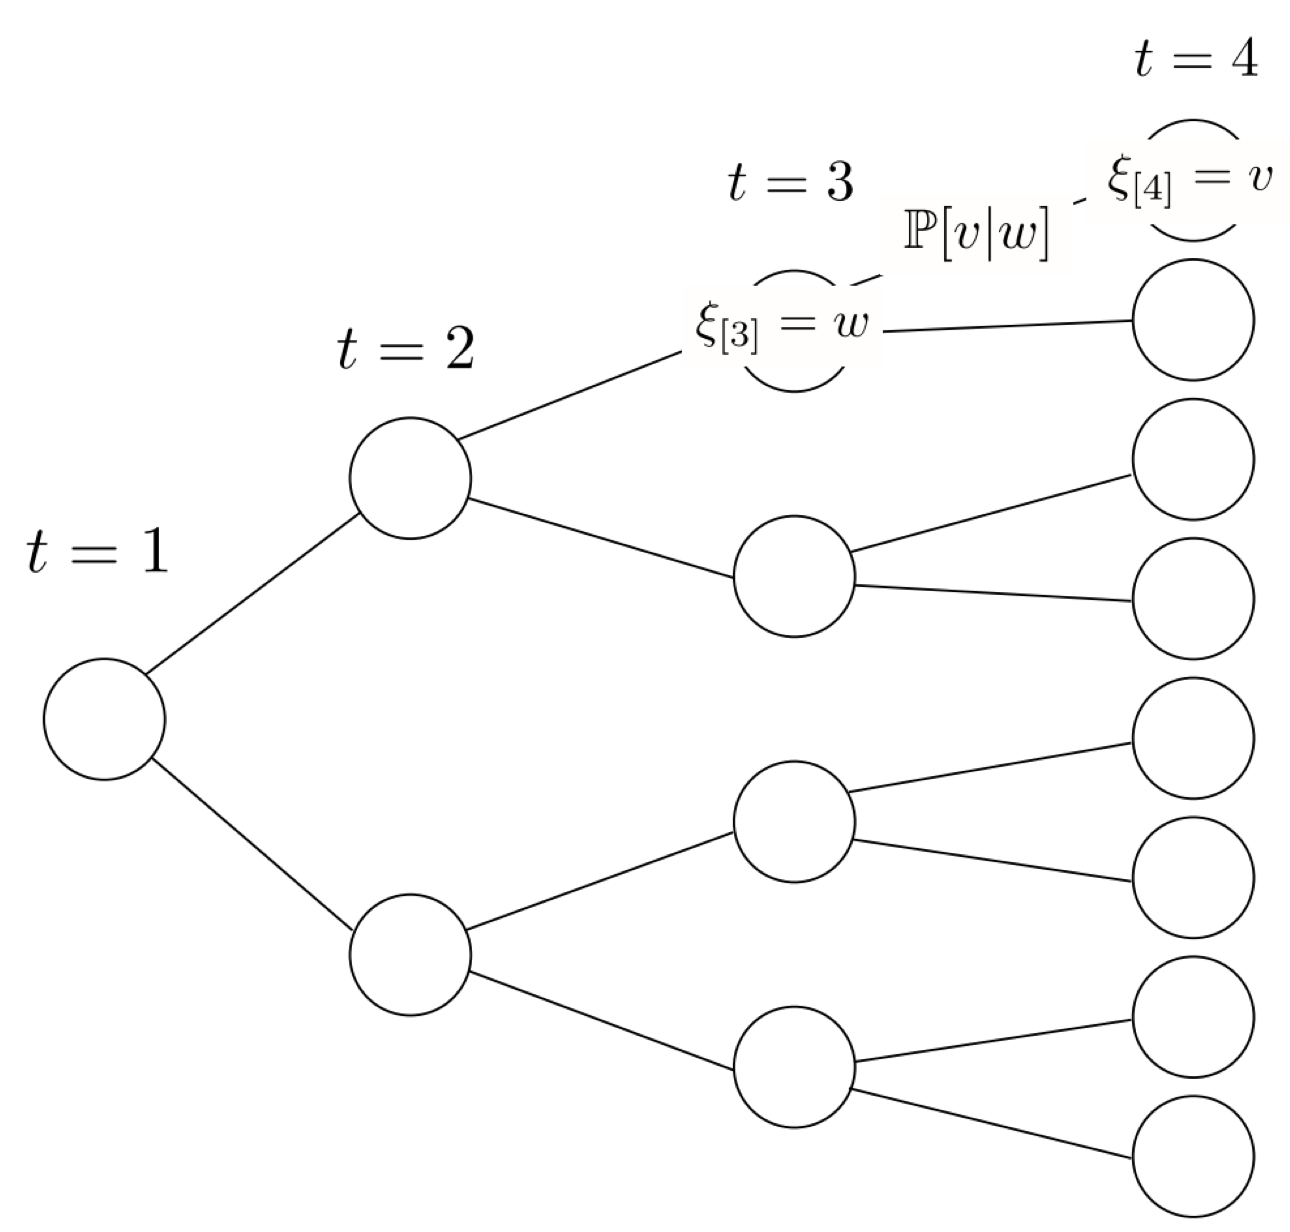
\includegraphics[width = .3\textwidth]{img/tree.png}
\end{figure}
\subsection{Lattice}
A lattice is a graphical representation of a Markov process $\{\xi_t\}_{t\in \Z}$, where the nodes are the realizations $\xi_t$ and the edges correspond to the transitions from $\xi_t$ to $\xi_{t+1}$. 
\begin{figure}[H]
	\centering 
	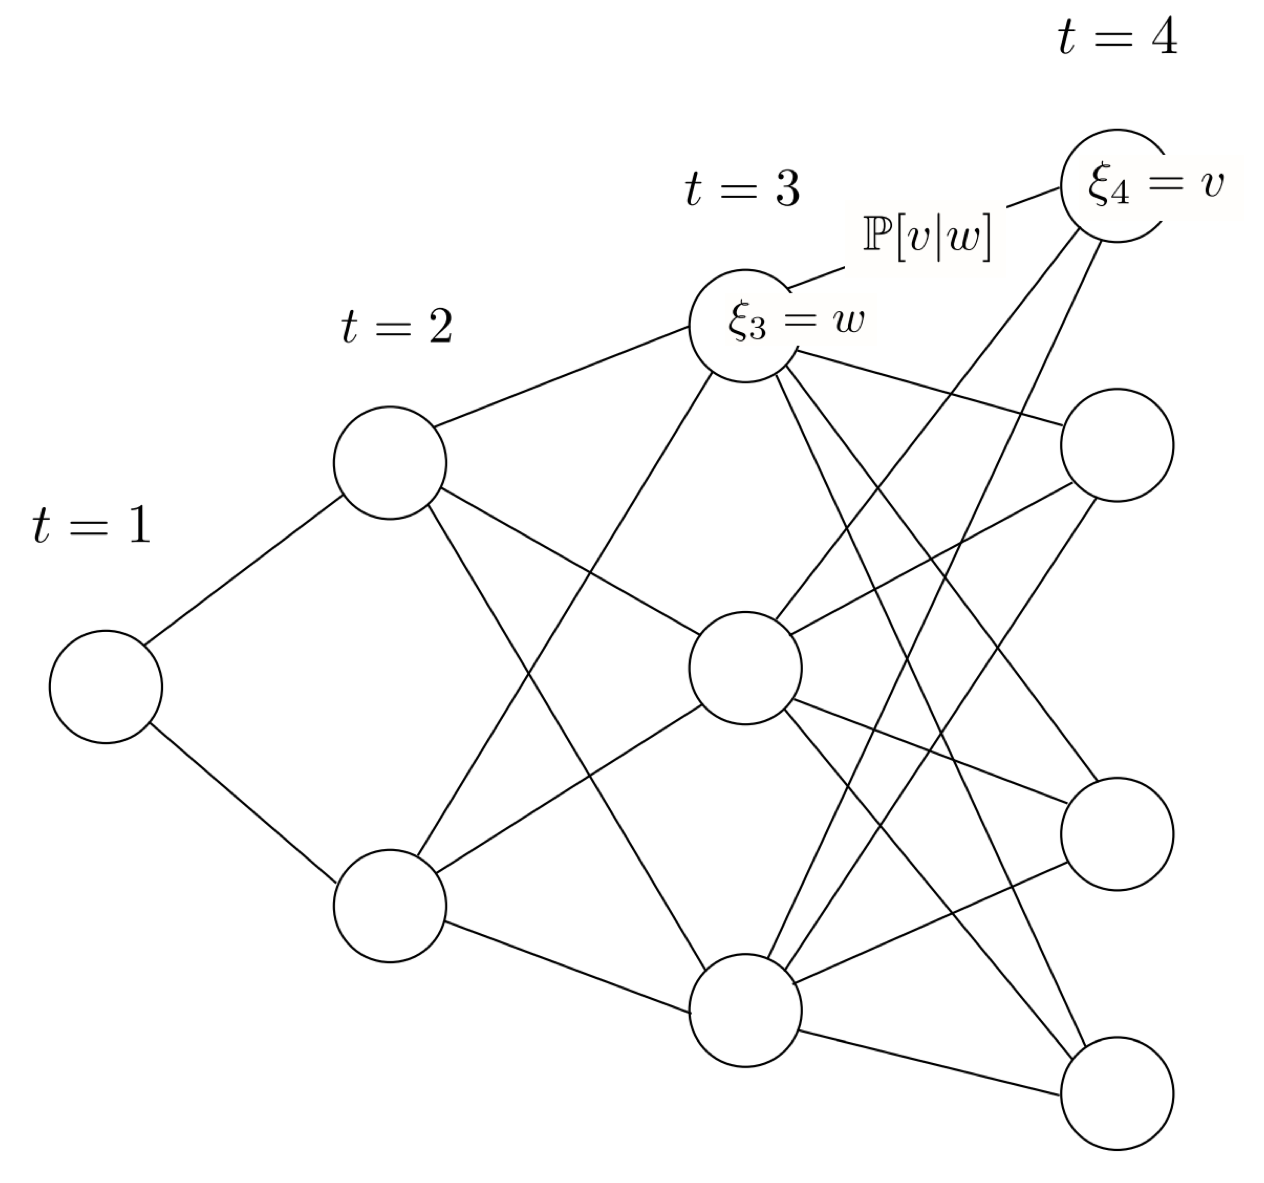
\includegraphics[width = .3\textwidth]{img/lattice.png}
\end{figure}
\subsection{Serial Independence}
A process satisfies serial independence if, for every stage $t$, $\xi_t$ has a probability distribution that does not depend on the history of the process. Thus, the probability measure is 
\begin{equation}
	\P\left[\xi_t(\omega)=i\left|\xi_{[t-1]}(\omega)\right.\right] = p_t(i) \qquad \forall \ \xi_{[t-1]}\in\Xi_{[t-1]}, i\in\Xi_t
\end{equation}
\section{Multi Stage Stochastic Linear Program}
\subsection{Notation}
\begin{itemize}
	\item Probability space: $(\Omega, 2^\Omega, \P)$ with filtration $\{\A\}_{t\in \{1, \dots, H\}}$
	\item $c_t(\omega) \in \R^{n_t}$: cost coefficients
	\item $h_t(\omega) \in \R^{m_t}$: right-hand side parameters
	\item $W_t(\omega) \in \R^{m_t \times n_t}$: coefficients of $x_t(\omega)$
	\item $T_{t-1}(\omega) \in \R^{m_t \times n_{t-1}}$: coefficients of $x_{t-1}(\omega)$
	\item $x_t(\omega)$: set of state and action variables in period $t$
	\item We implicitly enforce non-anticipativity by requiring that $x_t$ and $\xi_t$ are adapted to filtration $\{\mathcal{A}\}_{t\in \{1, \dots, H\}}$ 
	\item $\forall A \in \mathcal{A}_k \setminus \mathcal{A}_{k-1}, \: x_t(\omega_1)=x_t(\omega_2) \: \forall\omega_1,\omega_2 \in A$
\end{itemize}
\subsection{General formulation of the MSLP}
The extended formulation of the MSLP is: 
\begin{equation}
	\begin{aligned}
		&\min c_1^Tx_1 + \E[c_2(\omega)^T x_2(\omega)+ \dots + c_H(\omega)^Tx_H(\omega)]\\
		&s.t. \quad W_1x_1 = h_1\\
		&T_1(\omega)x_1 + W_2(\omega)x_2(\omega) = h_2(\omega), \omega \in \Omega\\
		&\qquad \qquad \vdots\\
		&T_{t-1}(\omega)x_{t-1}(\omega) + W_t(\omega)x_t(\omega) = h_t(\omega), \omega \in \Omega\\
		&\qquad \qquad \vdots\\
		&T_{H-1}(\omega)x_{H-1}(\omega) + W_H(\omega)x_H(\omega) = h_H(\omega), \omega \in \Omega\\
		&x_1 \geq 0, x_t(\omega) \geq 0, t=2, \dots, H
	\end{aligned}
\end{equation}
We can now consider two specific instantiations of the MSLP: the scenario tree (MSLP-ST) and the lattice (MSLP-L). Using these notations:
\begin{itemize}
	\item $\omega_t \in S_t$ : index in the support $\Xi_t$ of random input $\xi_t$
	\item $\omega_{[t]} \in S_1 \times \dots \times S_t$ (interpretation: index in $\Xi_{[t]} = \Xi_1 \times \dots \times \Xi_t$, which is the history of realizations, up to period $t$)
\end{itemize}
\subsection{Scenario Tree formulation}
\begin{equation}
	 \begin{aligned}
		&\min c_1^Tx_1 + \E\left[c_2(\omega_{[2]})^T x_2(\omega_{[2]})+ \dots + c_H(\omega_{[H]})^Tx_H(\omega_{[H]})\right]\\
		&s.t. \quad W_1x_1 = h_1\\
		&T_1(\omega_{[2]})x_1 + W_2(\omega_{[2]})x_2(\omega_{[2]}) = h_2(\omega_{[2]}), \omega_{[2]} \in S_1 \times S_2\\
		&\qquad \qquad \vdots\\
		&T_{t-1}(\omega_{[t]})x_{t-1}(\omega_{[t-1]}) + W_t(\omega_{[t]})x_t(\omega_{[t]}) = h_t(\omega_{[t]}), \omega_{[t]} \in S_1 \times \dots \times S_t\\
		&\qquad \qquad \vdots\\
		&T_{H-1}(\omega_{[H]})x_{H-1}(\omega_{[H-1]}) + W_H(\omega_{[H]})x_H(\omega_{[H]}) = h_H(\omega_{[H]}), \omega_{[H]} \in S_1 \times \dots \times S_H\\
		&x_1 \geq 0, x_t(\omega_{[t]}) \geq 0, t=2, \dots, H
	 \end{aligned}
\end{equation}
\subsection{Lattice formulation}
\begin{equation}
	\begin{aligned}
		&\min c_1^Tx_1 + \E\left[c_2(\omega_{2})^T x_2(\omega_{[2]})+ \dots + c_H(\omega_{H})^Tx_H(\omega_{[H]})\right]\\
		&s.t. \quad W_1x_1 = h_1\\
		&T_1(\omega_{2})x_1 + W_2(\omega_{2})x_2(\omega_{[2]}) = h_2(\omega_{2}), \omega_{[2]} \in S_1 \times S_2\\
		&\qquad \qquad \vdots\\
		&T_{t-1}(\omega_{t})x_{t-1}(\omega_{[t-1]}) + W_t(\omega_{t})x_t(\omega_{[t]}) = h_t(\omega_{t}), \omega_{[t]} \in S_1 \times \dots \times S_t\\
		&\qquad \qquad \vdots\\ 
		&T_{H-1}(\omega_{H})x_{H-1}(\omega_{[H-1]}) + W_H(\omega_{H})x_H(\omega_{[H]}) = h_H(\omega_{H}), \omega_{[H]} \in S_1 \times \dots \times S_H\\
		&x_1 \geq 0, x_t(\omega_{[t]}) \geq 0, t=2, \dots, H
	\end{aligned}
\end{equation}
\begin{itemize}
	\item [$\rightarrow$] Note: There exists some relations to other decision making problems such as statistical decision theory, dynamic programming, online optimization and stochastic control.
\end{itemize}

\chapter{Performance}
\section{Notation}
Using \eqref{eq:TSSLP_formulation}, let's define the following:
\begin{itemize}
	\item $z(x,\xi) = c^Tx+Q(x,\xi)+\delta(x|K_1)$
	\item $Q(x,\xi) = \displaystyle \min_y\{q(\omega)^Ty|W(\omega)y=h(\omega)-T(\omega)x\}$
	\item $K_1 = \{x|Ax=b,x\geq0\}$ is the set of feasible first-stage decisions
	\item $K_2(\omega)=\{x|\exists y\geq0:W(\omega)y=h(\omega)-T(\omega)x\}$ is the set of first-stage decisions that have a feasible reaction in the second stage for $\omega \in \Omega$
	\item It can be that $z(x,\xi) = + \infty$ (if $x \notin K_1 \cap K_2(\omega)$)
	\item It can be that $z(x,\xi) = - \infty$ (unbounded below)
\end{itemize}
\section{The expected value of perfect information}
There is 2 tactics:
\begin{itemize}
	\item \textbf{wait-and-see} value is the expected value of reacting with perfect
	foresight $x^*(\xi)$ to $\xi$: 
	\begin{equation}
		WS = \E[\displaystyle \min_x z(x,\xi)] = \E[z(x^*(\xi),\xi)]
	\end{equation}
	\item \textbf{here-and-now} value is the expected value of the recourse problem (remove non-anticipativity):
	\begin{equation}
		SP = \displaystyle \min_x \E[z(x,\xi)]
	\end{equation}
\end{itemize}
The \textbf{expected value of perfect information} is like the value of a perfect forecast for the future and is thus defined like this:
\begin{equation}
	EVPI = SP - WS
\end{equation}
\section{The value of the stochastic solution}
Here too there is 2 tactics:
\begin{itemize}
	\item \textbf{Expected value problem}
	\begin{equation}
		EV = \displaystyle \min_x z(x,\bar{\xi}) = \E[\xi]
	\end{equation}
	and it's \textbf{expected value solution} is noted $x^*(\bar{\xi})$
	\item \textbf{expected value of using the EV solution} measures the performance of $x^*(\bar{\xi})$:
	\begin{equation}
		EEV = \E[z(x^*(\bar{\xi}),\xi)]
	\end{equation}
\end{itemize}
% We also have $EEV \geq SP$.\\
The \textbf{value of the stochastic solution} is noted like this:
\begin{equation}
	VSS = EEV - SP
\end{equation}
\section{Basic inequalities}
\subsection{Crystal Ball}
For every $\xi$, we have $z(x^*(\xi),\xi) \leq z(x^*,\xi)$ where $x^*$ is the optimal solution to the stochastic program. And if we take the expectation of this inequality, we have $WS \leq SP$, because $WS$ is a relaxation. It explains that we can do better with a Crystal Ball. 
\subsection{Lazy solution}
Knowing that $x^*$ is the optimal solution of $\displaystyle \min_x \E[z(x,\xi)]$ and $x^*(\bar{\xi})$ is a solution but not necessarily optimal then we have $SP \leq EEV$, because:
\begin{equation}
	\displaystyle \min_x \E[z(x,\xi)] = SP \leq EEV = \E[z(x^*(\bar{\xi}),\xi)]
\end{equation}
\subsection{Link between all the values}
We know that:
\begin{itemize}
	\item $VSS \geq 0$
	\item $EVPI \geq 0$
	\item $VSS \leq EEV - EV$
	\item $EVPI \leq EEV -EV$
	\item If $EEV - EV = 0$ then $VSS = EVPI = 0$
\end{itemize}
and the inequalities can be summarized in the following diagram:
\begin{figure}[H]
	\centering
	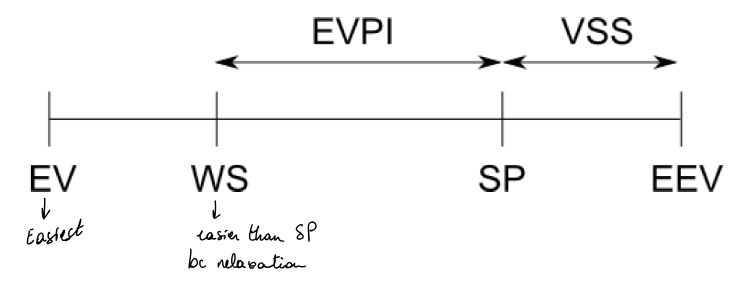
\includegraphics[scale=0.5]{img/link_ineq.png}
\end{figure}
\section{Bounds on EVPI and VSS}
First let's introduce the pairs subproblem of $\xi^r$ and $\xi^k$ is
\begin{equation}
	\begin{aligned}
		\min \: &z^P (x, \xi^r,\xi^k) = c^Tx + p^rq^Ty(\xi^r) + (1-p^r)q^Ty(\xi^k)\\
		s.t. \: &Ax = b\\
		&Wy(\xi^r) = \xi^r-Tx\\
		&Wy(\xi^k) = \xi^k-Tx\\
		&x,y\geq0
	\end{aligned}
\end{equation}
\begin{itemize}
	\item $(\bar{x}^k , \bar{y}^k , y(\xi^r ))$ denotes an optimal solution to the problem and zk is the optimal objective function value $z^P (\bar{x}^k , \bar{y}^k , y(\xi^k ))$
	\item $z^P (x, \xi^r , \xi^r)$ corresponds to the deterministic optimization against the
	reference scenario
	\item if $\xi^r \notin \Xi$, $p^r = 0$ and $z^P (x, \xi^r , \xi^k ) = z(x, \xi^k )$
\end{itemize}
The \textbf{sum of pairs expected value (SPEV)}:
\begin{equation}
	SPEV = \frac{1}{1-p^r} \sum_{k=1,k \neq r}^{K} p^k \min z^P(x, \xi^r,\xi^k)
\end{equation}
When $\xi^r \notin \Xi$ then $SPEV = WS$: When $p^r = 0, z^P(x,\xi^r,\xi^k)$ coincides with $z(x,\xi^k)$. Therefore $SPEV = \sum_{k=1}^{K} p^k \min_x z(x,\xi^k) = WS$.\\
We then know $WS \leq SPEV \leq SP$.
\subsection{Upper bound on SP: EVRS and EPEV}
\begin{itemize}
	\item The \textbf{expected value of the reference scenario} is $EVRS =  \E_\xi(\bar{x}^r,\xi)$, where $\bar{x}^r$ is the optimal solution to $z(x,\xi^r)$ 
	\item The \textbf{expectation of pairs of expected value} is defined as \\$EPEV = \min_{k=1,\dots,K\cup\{r\}}\E_\xi(\bar{x}^r,\xi)$ where $(\bar{x}^k,\bar{y}^k, y(\xi^K))$ is the optimal solution to the pairs subproblem of $\xi^r$ and $\xi^k$
\end{itemize}
As $SP,EPEV,EVRS$ are the optimal values of $\min_x \E_\xi z(x,\xi)$ over smaller feasible sets:
\begin{equation}
	SP \leq EPEV \leq EVRS
\end{equation}
Because
\begin{itemize}
	\item $SP$: $x \in K_1 \cap K_2$
	\item $EPEV$: $x \in K_1 \cap K_2 \cap \{\bar{x}^k,k=1,\dots,K\cup\{r\}\}$
	\item $EVRS$: $x \in \bar{x}^r \cap K_1 \cap K_2$
\end{itemize}

\end{document}